Ontology is a concept originating from Philosophy, referring to the
study of the nature of being, as well as the basic categories of being
and their relations~\cite{noy2001ontology}. In recent decades, it has
become a branch in Information Science for representing the knowledge
in a particular domain. In this context, 
%an {\bf ontology} consists of
%four components: {\em classes or called concepts}, {\em properties},
%{\em restrictions}, and {\em individuals}. 
an ontology is a formal explicit
description of a domain's knowledge, including concepts (or classes), properties of each concept 
(or relations)
%, constraints on the properties (or restrictions), 
and individuals (or instances of classes)~\cite{staab2013handbook}.
An ontology is often visualized as a graph in which nodes indicate
concepts and edges indicate relations between concepts. It is often
represented in some standard three-tuple format as we will described
later in this section.  Developing an ontology for a domain has many
benefits, including 1) making domain knowledge explicit to expose what
is known and what is unknown, 2) enabling knowledge interoperability
by providing a common taxonomy and vocabulary, 3) providing knowledge
reuse since the ontology is a persistent knowledge base, and 4)
facilitating knowledge validation and reasoning using existing
inference engines (or reasoners).
%With an ontology, a user can
%define some individual instances of some classes in the domain.  
%An
%ontology together with a set of individual instances of classes
%constitutes a knowledge base of a domain.

Figure~\ref{fig:wine} shows an example borrowed from an introductory
article of ontology~\cite{noy2001ontology}. A class (e.g., ``Winery'')
describes concepts in a domain. A class can have subclasses,
representing the ``kind of'' relations among concepts (e.g., ``red
wine'' may be a subclass of ``wine'').  A class can have many
individual instances (e.g., ``Chateau Lafite Rothschild Pauillac'' is
an instance of the class ``Pauillac''). A property describes the
attribute of a class or instance. It is usually represented as an edge
between classes or instances. For instance, the ``maker'' property in
Figure~\ref{fig:wine} shows that the maker of ``Chateau Lafite
Rothschild Pauillac'' is ``Chateau Lafite Rothschild''. A property may
have some constraints, which describe the value type, allowed values,
the number of the values (cardinality), and other features of the
values which the property can take.

\begin{figure}[hb]
\centering
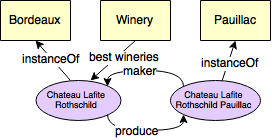
\includegraphics[width=.4\columnwidth]{graph/wine.png}
\caption{An example ontology for the domain of winery.}
\label{fig:wine}
\end{figure}
%\TODO{This is a bad example, not familiar domain with foreign names. Changed it to Person, Parents, Human etc to shown similar nodes and edge, matching the text later on}

% I want to quickly introduce DL and OWL.
The theory foundation of ontology is Description Logic (DL)~\cite{krotzsch2012description}, a family of formal knowledge representation languages for formal reasoning on the concepts of a domain. 
DL is expressive enough to build sophisticated knowledge bases while still supporting efficient inference.
It has a popular standardized dialect, Web Ontology
Language or OWL~\cite{mcguinness2004owl}. 
%Programming languages based on Description Logics (DL) are often used
%for representing an ontology~\cite{krotzsch2012description}. 
DL allows the use of {\em axioms} to describe a knowledge
base. For instance, an axiom \textsf{Person(Alex)} describes that
``Alex'' is an instance of class ``Person'',
and $\mathsf{Person}\sqsupseteq \mathsf{Human}$ describes the
subsumption relationship between concept \textsf{Person} and concept
\textsf{Human}. DL languages could use different
grammars. Conventionally, a simple yet uniform format to represent axioms is \textsf{(subject, property, object)} triple. Axioms in DL
languages can all be mapped to such a format. For instance, in
\textsf{Person(Alex)}, ``Alex'' is the subject, ``instance of'' is the
property, and ``Person'' is the object. Visually, it is an ``instance
of'' edge flowing from the ``Alex'' node to the ``Person'' node in an
ontology graph.

%For the generic form of knowledge representation offered by Ontology,
%automatic inferences on the knowledge of a domain becomes possible.
Through decades of development, a large body of tools 
(e.g., Stanford Protege~\cite{gennari2003evolution}, SWI-Prolog Semantic Web Library~\cite{wielemaker2011}, etc.)
%\TODO{add citations for DL reasoners such as SWI-Prolog, Pellet,
%Racer, FaCT++, HermiT, etc}
have been developed for creating ontologies and automatic reasoning upon an ontology-based
knowledge base, which enables automatic questions-and-answers,
consistency check of the knowledge base, derivation of new knowledge,
and so on.

Like declarative program analysis, most of these tools leverage logic
programming languages (e.g., Prolog) for inferences. In logical
programming, a program is composed of a list of rules written in the
form of \emph{clauses}:
\[
\mathsf{H \mbox{:-}  B_1, \dots, B_n.}
\]
which reads as 
\[
\textsf{H is true if } \mathsf{B_1} \textsf{ is true and ... } \mathsf{B_n} \textsf{ is true.}
\]

H is called the \emph{head} of the rule and $\mathsf{B_1, \dots, B_n}$
is called the body. When the body is empty, the rule
becomes \emph{fact} such as $\mathsf{variable(a)}$. 

%\TODO{Queries and how they are resolved by the underneath inference
%  engine of a logic language implementation.}





